\textbf{\uline{Exemplo 03:}}
	\begin{center}
		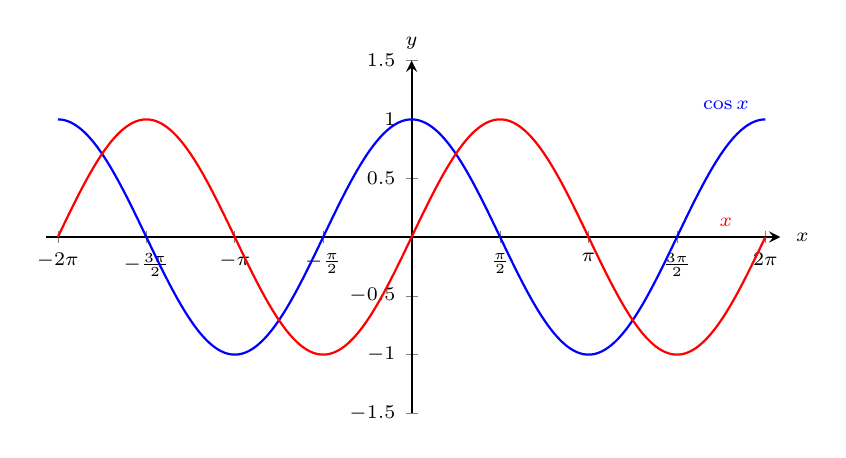
\begin{tikzpicture}[font=\scriptsize]
			\begin{axis}[thick,smooth,axis lines=middle,width=0.9\textwidth,
				height=0.5\textwidth,
				xmin=-6.5,xmax=6.55,ymin=-1.5,ymax=1.5,
				every axis x label/.style={
					at={(ticklabel* cs:1.03)}},
				every axis y label/.style={
					at={(ticklabel* cs:1.05)}},
				xtick={-6.28318, -4.7123889, ..., 6.28318},
				xticklabels={$-2\pi$, $-\frac{3\pi}{2}$, $-\pi$   , $-\frac{\pi}{2}$,,  $\frac{\pi}{2}$,  $\pi$   , $\frac{3\pi}{2}$, $2\pi$},
				xlabel=$x$,ylabel=$y$,ytick distance=0.5,samples=400]
				\addplot[blue,domain=-2*pi:2*pi] {cos(deg(x))} node[above,xshift=-0.5cm]{$\cos x$};
				\addplot[red,domain=-2*pi:2*pi] {sin(deg(x))} node[above,xshift=-0.5cm]{$\sen x$};
			\end{axis}
		\end{tikzpicture}
	\end{center}